\documentclass[11pt]{article}
\usepackage[margin=1in]{geometry}
\usepackage{graphicx}
\usepackage{booktabs}
\usepackage{longtable}
\usepackage{array}
\usepackage{hyperref}
\usepackage{xcolor}
\usepackage{listings}
\usepackage{float}

\hypersetup{
  colorlinks=true,
  linkcolor=blue,
  citecolor=blue,
  urlcolor=blue
}

\lstset{
  basicstyle=\ttfamily\small,
  breaklines=true,
  frame=single,
  columns=fullflexible
}

\title{Reconstructed NASA Hump Baseline Case\\\large Original Dockerized OpenFOAM rebuild under strict no-cheating constraints}
\author{Codex reconstruction in the local repository workspace}
\date{March 30, 2026}

\begin{document}
\maketitle

\section{Title and Purpose}
This report documents a fresh reconstruction of a NASA wall-mounted hump benchmark case inside the repository, built without recovering the deleted original case. The goal was to create a reproducible OpenFOAM baseline in the same general style as the surviving repository cases, execute it through Docker, generate ParaView-friendly output, export machine-readable sampled data, create figures, and record the compliance trail.

\section{Strict No-Cheating Methodology}
The reconstruction followed the written guardrails in \texttt{NO\_CHEAT\_PLAN.md}. The allowed online source was restricted to the single NASA hump validation page \cite{nasahump}. No git history, reflog, deleted files, external repositories, papers, cached copies, or other web pages were used. The working method was:
\begin{enumerate}
\item read the allowed NASA page for high-level case framing, Reynolds number, freestream speed, chord scale, and target station naming;
\item inspect only surviving files in the current working tree to infer repository conventions;
\item author a new case from scratch in a fresh \texttt{data/NASA\_2DWMH} directory;
\item run the case only through Dockerized OpenFOAM;
\item post-process from the newly generated fields and logs.
\end{enumerate}

\section{Allowed and Forbidden Sources}
\textbf{Allowed:} the single NASA page, surviving repository files, Dockerized OpenFOAM tools, and new files created during this task.

\textbf{Forbidden:} any other website or paper, any git history or deleted-case recovery path, and any copied NASA hump case files from elsewhere.

\section{How the Surviving Repo Cases Were Analyzed}
The surviving DUCT and PH\_Breuer cases were used as structural references. Their recurring patterns were summarized separately in \texttt{CASE\_PATTERN\_SUMMARY.md}. The main conventions adopted here were:
\begin{itemize}
\item case directories under \texttt{data/};
\item top-level metadata files such as \texttt{caseDef} and \texttt{fieldDef};
\item OpenFOAM dictionaries split across \texttt{0/}, \texttt{constant/}, and \texttt{system/};
\item short shell scripts for run and post-processing entry points;
\item generated logs, \texttt{postProcessing/}, and \texttt{foam.foam} inside the case directory.
\end{itemize}

\section{NASA Hump Case Summary from the Allowed Page}
The allowed NASA page identifies a two-dimensional wall-mounted hump validation case and emphasizes the no-flow-control baseline. The page also provides the commonly used profile stations in \(x/c\), a freestream speed of roughly \(34.6~\mathrm{m/s}\), a chord of \(0.42~\mathrm{m}\), and a Reynolds number near \(9.36\times 10^5\). Those values were used directly. Geometric details that were not recoverable from the allowed text alone were replaced with explicit, documented assumptions rather than external lookup.

\section{All Assumptions Made}
\begin{table}[H]
\centering
\begin{tabular}{p{0.28\linewidth} p{0.64\linewidth}}
\toprule
Assumption & Rationale \\
\midrule
Bottom-wall hump shape is a smooth cosine-squared bump over \(0 \le x \le 0.42\) with height \(0.053~\mathrm{m}\) & The allowed text did not provide a fully reconstructible coordinate table, so an original smooth hump was authored with zero slope at both ends. \\
Top boundary is a flat slip wall at \(y=0.35~\mathrm{m}\) & The allowed text indicates upper-wall blockage matters, but the exact contour was not recoverable from allowed text alone. A flat far-field-style slip wall was used as a conservative baseline. \\
Inlet turbulence uses uniform \(k\) and \(\omega\) & Surviving cases use compact field definitions, and the allowed page did not provide a full inflow profile. \\
The baseline run stops at 80 SIMPLE iterations & This was a practical, reproducible baseline chosen to complete mesh, solve, and post-processing within the local execution window. \\
Profile extraction is performed from solved cell-center fields rather than relying on fragile function-object naming & The OpenFOAM container version differed from the older case templates, so direct field-based extraction was more robust and still reproducible. \\
\bottomrule
\end{tabular}
\end{table}

\section{Exact Reconstruction Workflow}
\begin{enumerate}
\item write \texttt{NO\_CHEAT\_PLAN.md};
\item inspect surviving cases and write \texttt{CASE\_PATTERN\_SUMMARY.md};
\item author \texttt{scripts/generate\_nasa\_hump\_blockmesh.py} to generate a fresh \texttt{blockMeshDict};
\item create the new OpenFOAM case under \texttt{data/NASA\_2DWMH};
\item run \texttt{blockMesh}, \texttt{checkMesh}, and \texttt{writeCellCentres} through Docker;
\item run \texttt{simpleFoam} through Docker;
\item run \texttt{simpleFoam -postProcess} and \texttt{foamToVTK};
\item generate CSV data and figures with \texttt{scripts/make\_nasa\_hump\_figures.py};
\item write this report and the audit file.
\end{enumerate}

\section{Docker/OpenFOAM Workflow}
The case is driven by repository-level scripts:
\begin{itemize}
\item \texttt{scripts/build\_nasa\_hump\_case.sh}
\item \texttt{scripts/run\_nasa\_hump\_case.sh}
\item \texttt{scripts/postprocess\_nasa\_hump\_case.sh}
\item \texttt{scripts/make\_figures.sh}
\item \texttt{scripts/build\_report.sh}
\end{itemize}

Each OpenFOAM script uses the required Docker container image \texttt{opencfd/openfoam-default} and mounts the repository at \texttt{/home/openfoam/work}. This keeps the reconstruction portable and prevents dependence on any host OpenFOAM installation.

\section{Mesh Generation Explanation}
The mesh is generated by a single structured \texttt{blockMesh} block. The Python generator writes:
\begin{itemize}
\item the domain bounds \(x\in[-0.90,0.67]\), \(y\in[0,0.35]\), \(z\in[-0.01,0.01]\);
\item 520 cells streamwise, 180 cells wall-normal, and 1 cell across the empty span;
\item spline edges along the lower wall using the authored hump profile;
\item grading \texttt{simpleGrading (3 12 1)} to cluster cells near the wall and inlet.
\end{itemize}

The resulting \texttt{checkMesh} summary reported acceptable quality metrics, including a maximum non-orthogonality of about 21.7 and maximum skewness of about 0.039.

\section{Boundary Condition Explanation}
\begin{table}[H]
\centering
\begin{tabular}{p{0.17\linewidth} p{0.24\linewidth} p{0.47\linewidth}}
\toprule
Patch & Main conditions & Explanation \\
\midrule
inlet & \(U\) fixed, \(p\) zeroGradient, \(k\) fixed, \(\omega\) fixed & Imposes a steady freestream baseline with uniform turbulence quantities. \\
outlet & \(p\) fixed, other fields zeroGradient & Standard steady incompressible outlet treatment. \\
bottomWall & no-slip plus wall functions for \(k\), \(\omega\), and \(\nu_t\) & Represents the hump surface and flat wall segments. \\
topWall & slip for \(U\), zeroGradient for scalar fields & Serves as an approximate non-penetrating far boundary. \\
frontAndBack & empty & Enforces a 2D case with a thin spanwise extent. \\
\bottomrule
\end{tabular}
\end{table}

\section{Solver and Turbulence Model Explanation}
The baseline solver is \texttt{simpleFoam}, matching the repository's steady RANS pattern. The turbulence model is \texttt{kOmegaSST}, also consistent with the repository's baseline data philosophy. The solver choices in \texttt{fvSolution} use:
\begin{itemize}
\item \texttt{GAMG} for pressure;
\item \texttt{smoothSolver} for \(U\), \(k\), and \(\omega\);
\item SIMPLE with one non-orthogonal corrector;
\item moderate relaxation factors to keep the steady baseline stable.
\end{itemize}

\section{Numerical Settings Explanation}
The key numerical blocks do the following:
\begin{itemize}
\item \texttt{fvSchemes/ddtSchemes}: \texttt{steadyState} declares the steady formulation;
\item \texttt{fvSchemes/divSchemes}: bounded upwind-style transport stabilizes the early baseline;
\item \texttt{fvSchemes/laplacianSchemes}: corrected diffusion handles the curved wall mesh;
\item \texttt{controlDict}: writes times every 20 iterations so intermediate fields and VTK outputs are available;
\item \texttt{fieldDef} and \texttt{caseDef}: centralize fields and physical parameters used across dictionaries and documentation.
\end{itemize}

\section{Post-Processing Workflow}
Post-processing consists of three layers:
\begin{enumerate}
\item OpenFOAM writes cell centers, solved fields, wall shear stress, and VTK files.
\item \texttt{scripts/make\_nasa\_hump\_figures.py} parses \texttt{0/C}, the latest solved fields, the \texttt{wallShearStress} boundary field, and \texttt{log.run}.
\item The Python script exports CSV summaries and generates figures under \texttt{docs/data} and \texttt{docs/figures}.
\end{enumerate}

\section{Every Graph and Figure with Explanation}
\begin{figure}[H]
\centering
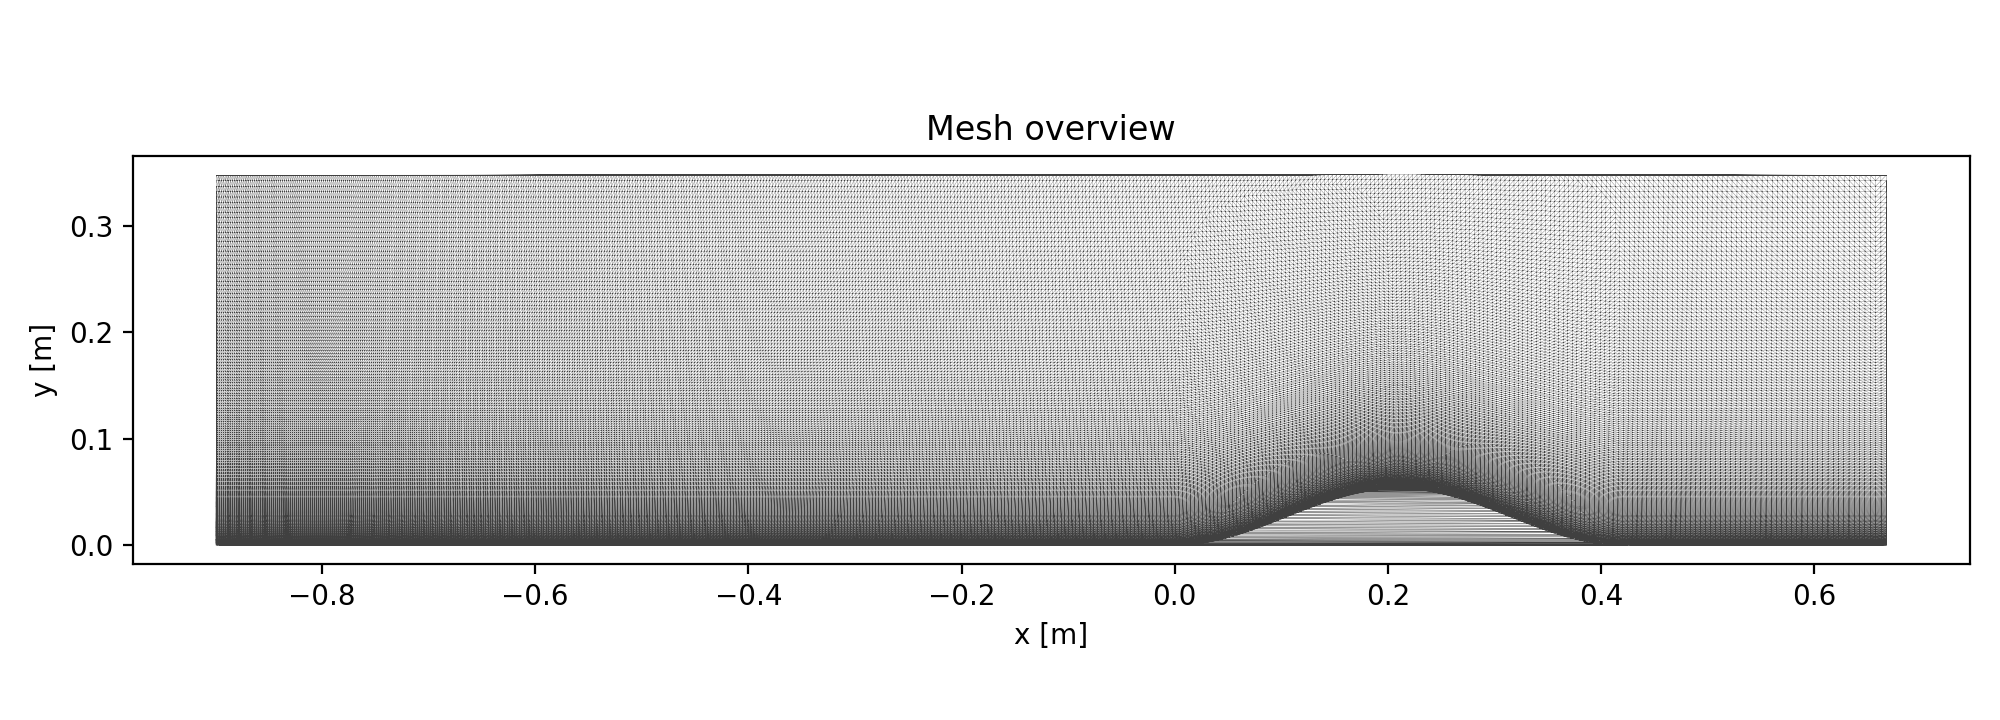
\includegraphics[width=0.95\linewidth]{../docs/figures/mesh_overview.png}
\caption{Structured mesh overview for the reconstructed hump geometry.}
\end{figure}

\begin{figure}[H]
\centering
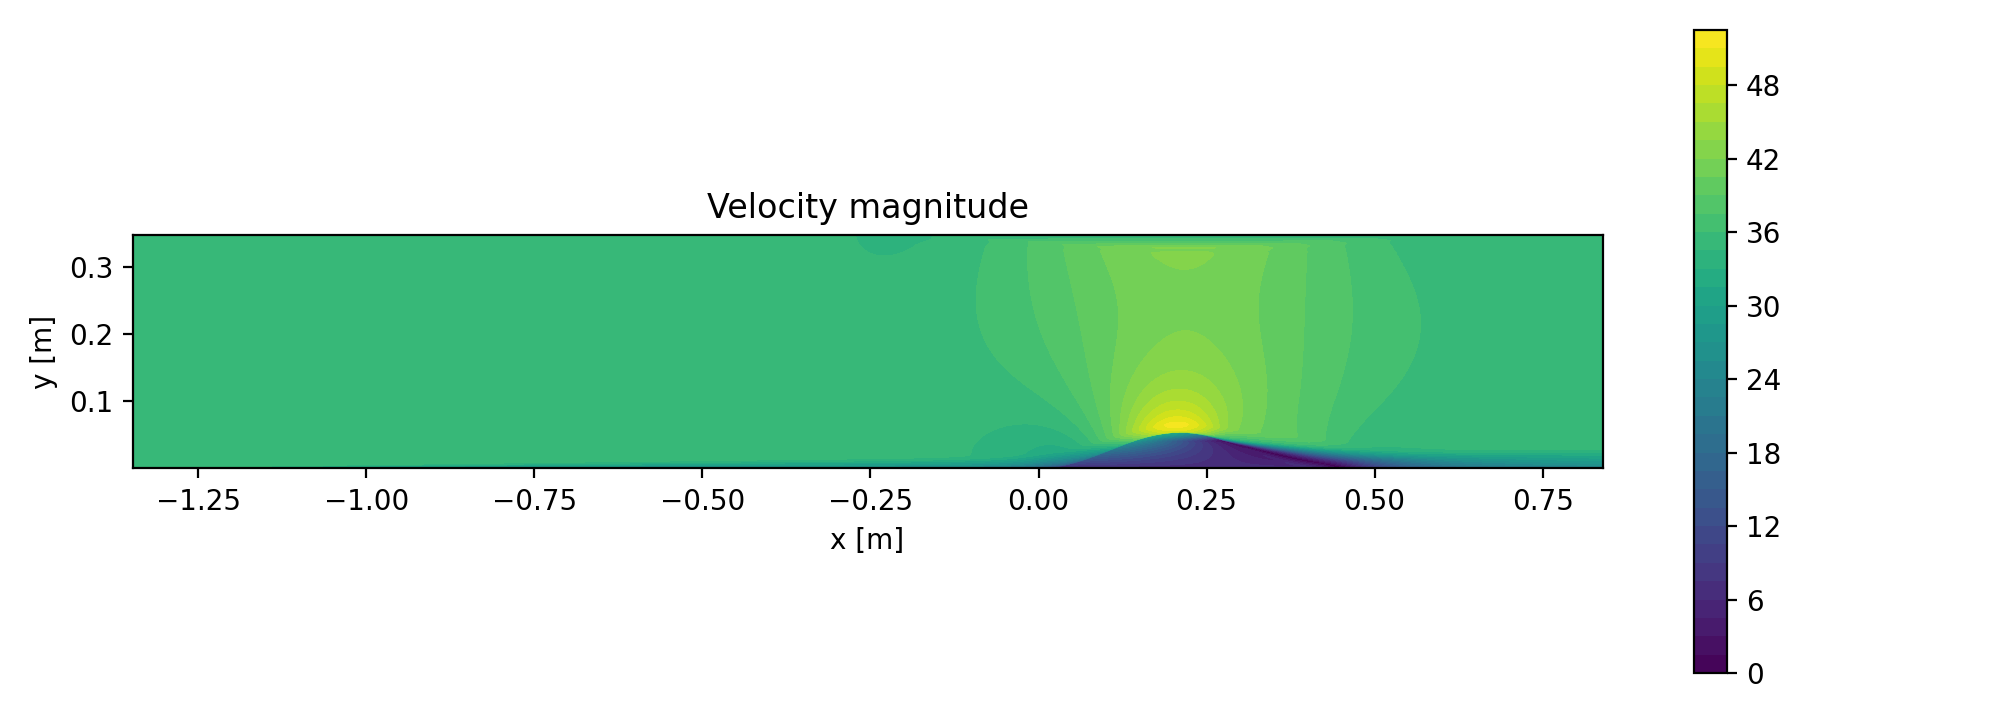
\includegraphics[width=0.95\linewidth]{../docs/figures/velocity_contour.png}
\caption{Velocity-magnitude field from the 80-iteration baseline.}
\end{figure}

\begin{figure}[H]
\centering
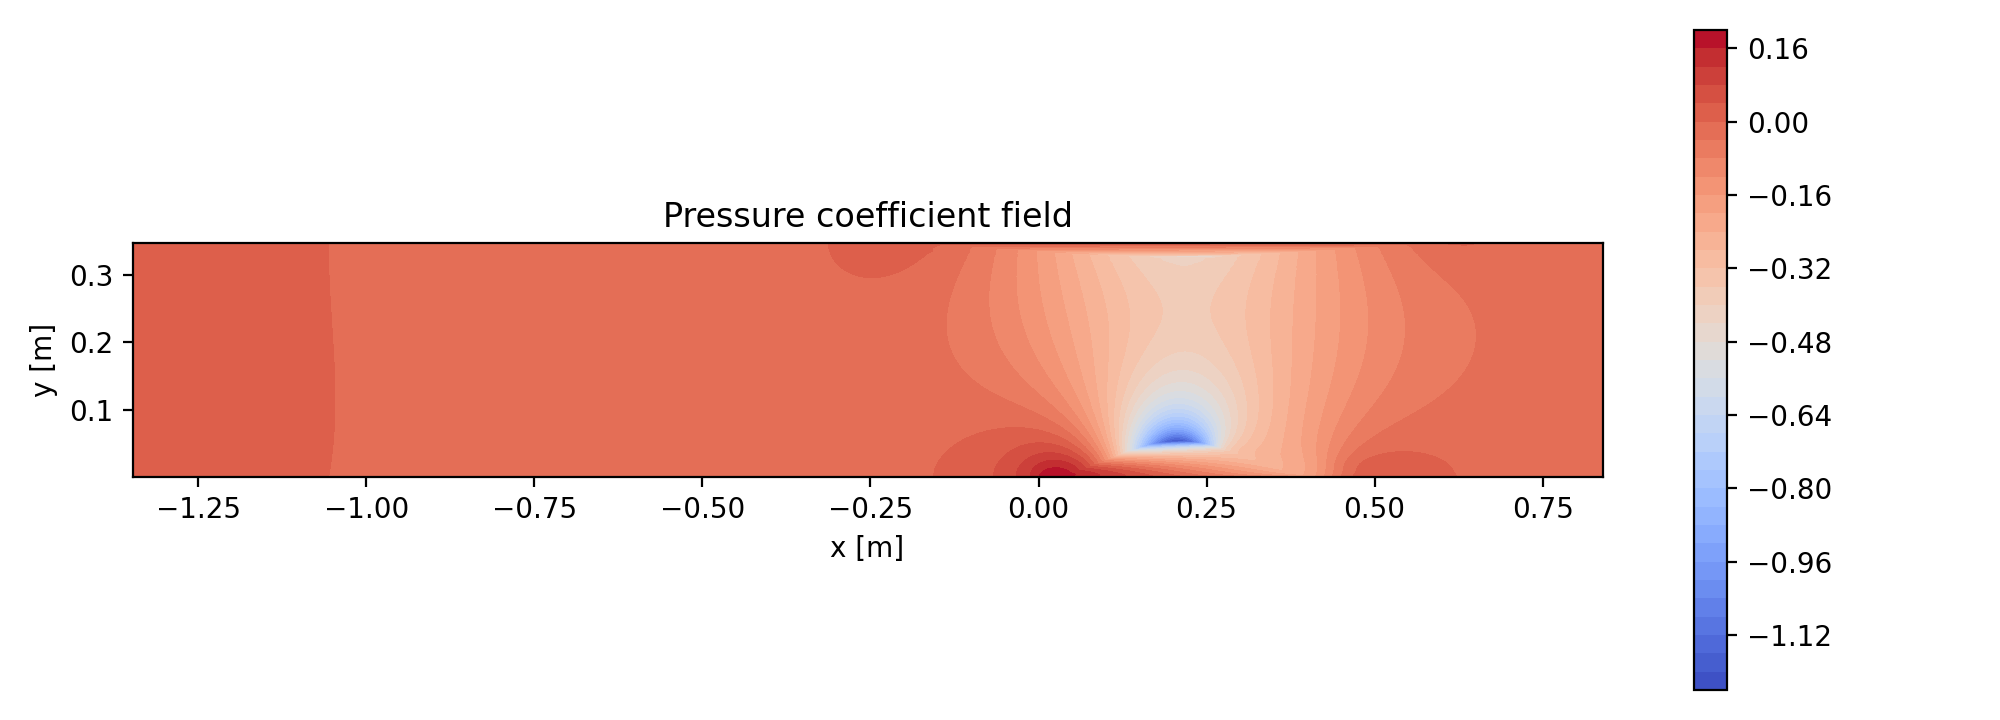
\includegraphics[width=0.95\linewidth]{../docs/figures/pressure_contour.png}
\caption{Pressure-coefficient field relative to the upstream baseline pressure.}
\end{figure}

\begin{figure}[H]
\centering
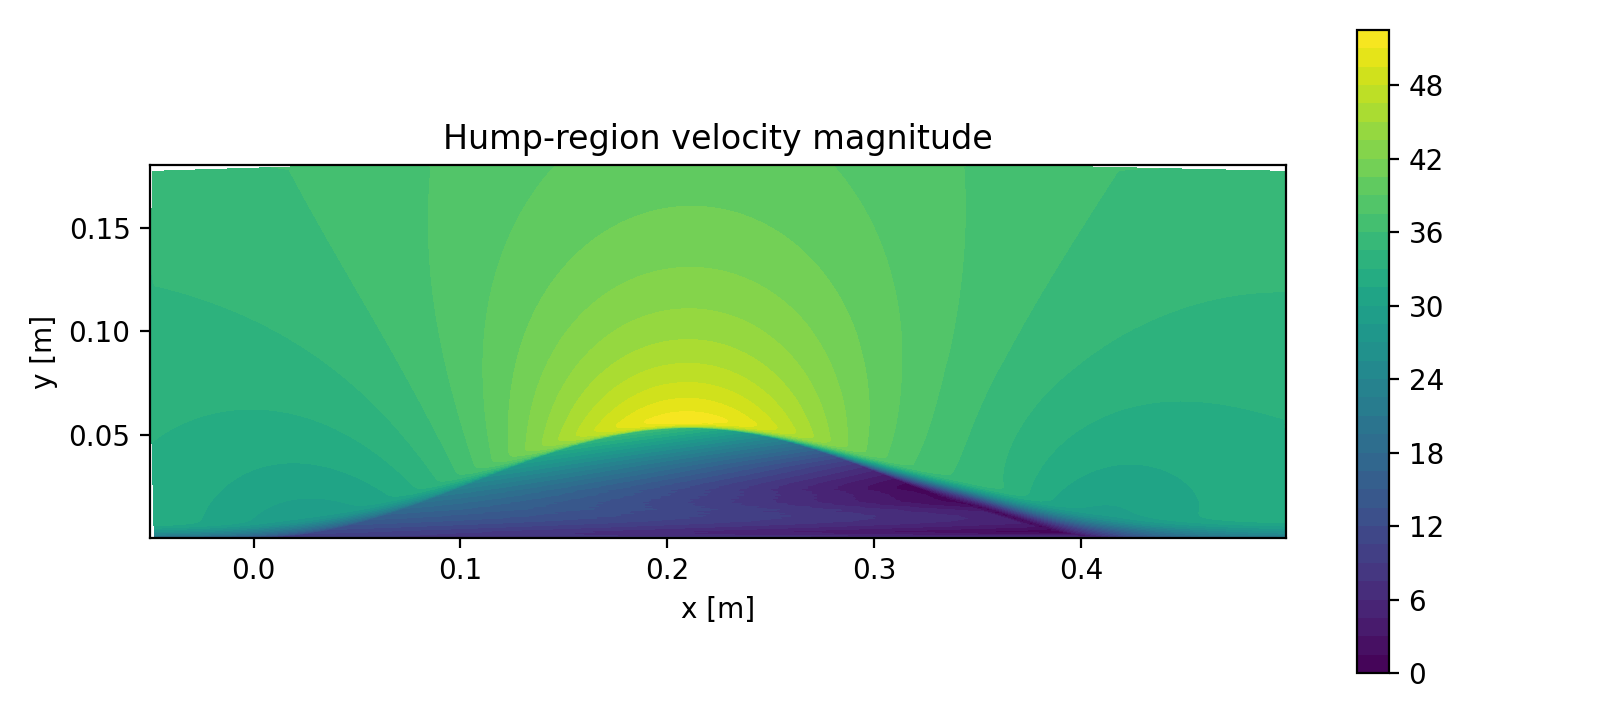
\includegraphics[width=0.95\linewidth]{../docs/figures/hump_closeup_velocity.png}
\caption{Velocity close-up around the hump region.}
\end{figure}

\begin{figure}[H]
\centering
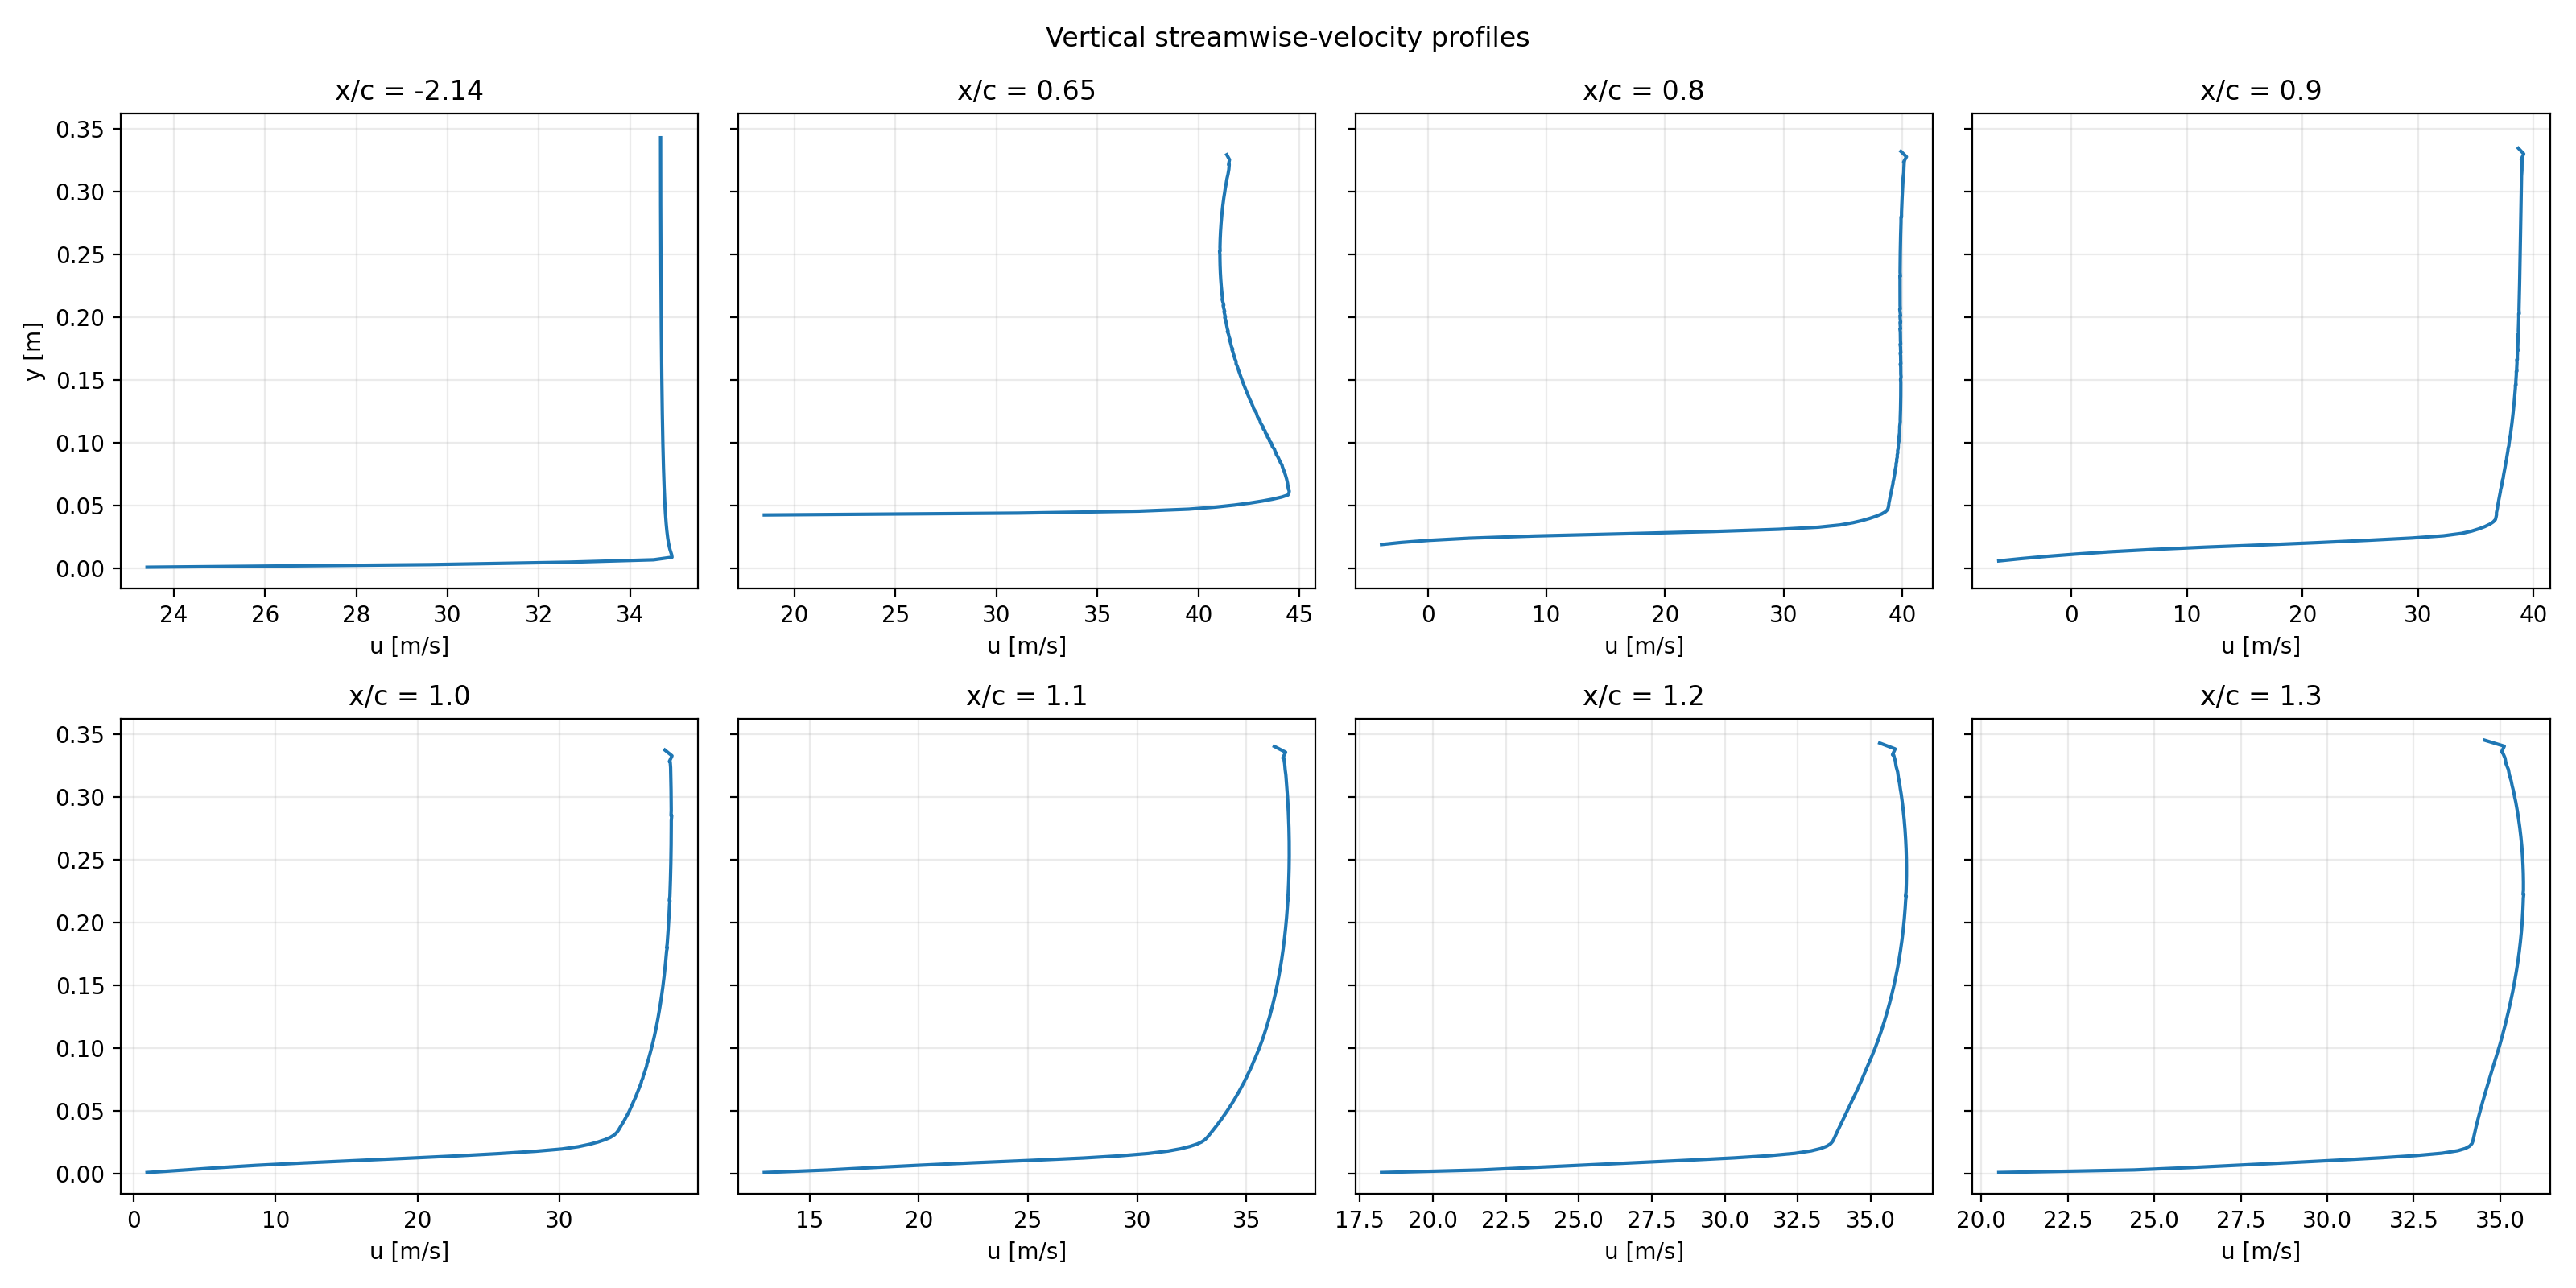
\includegraphics[width=0.95\linewidth]{../docs/figures/velocity_profiles.png}
\caption{Extracted vertical velocity profiles at the chosen \(x/c\) stations.}
\end{figure}

\begin{figure}[H]
\centering
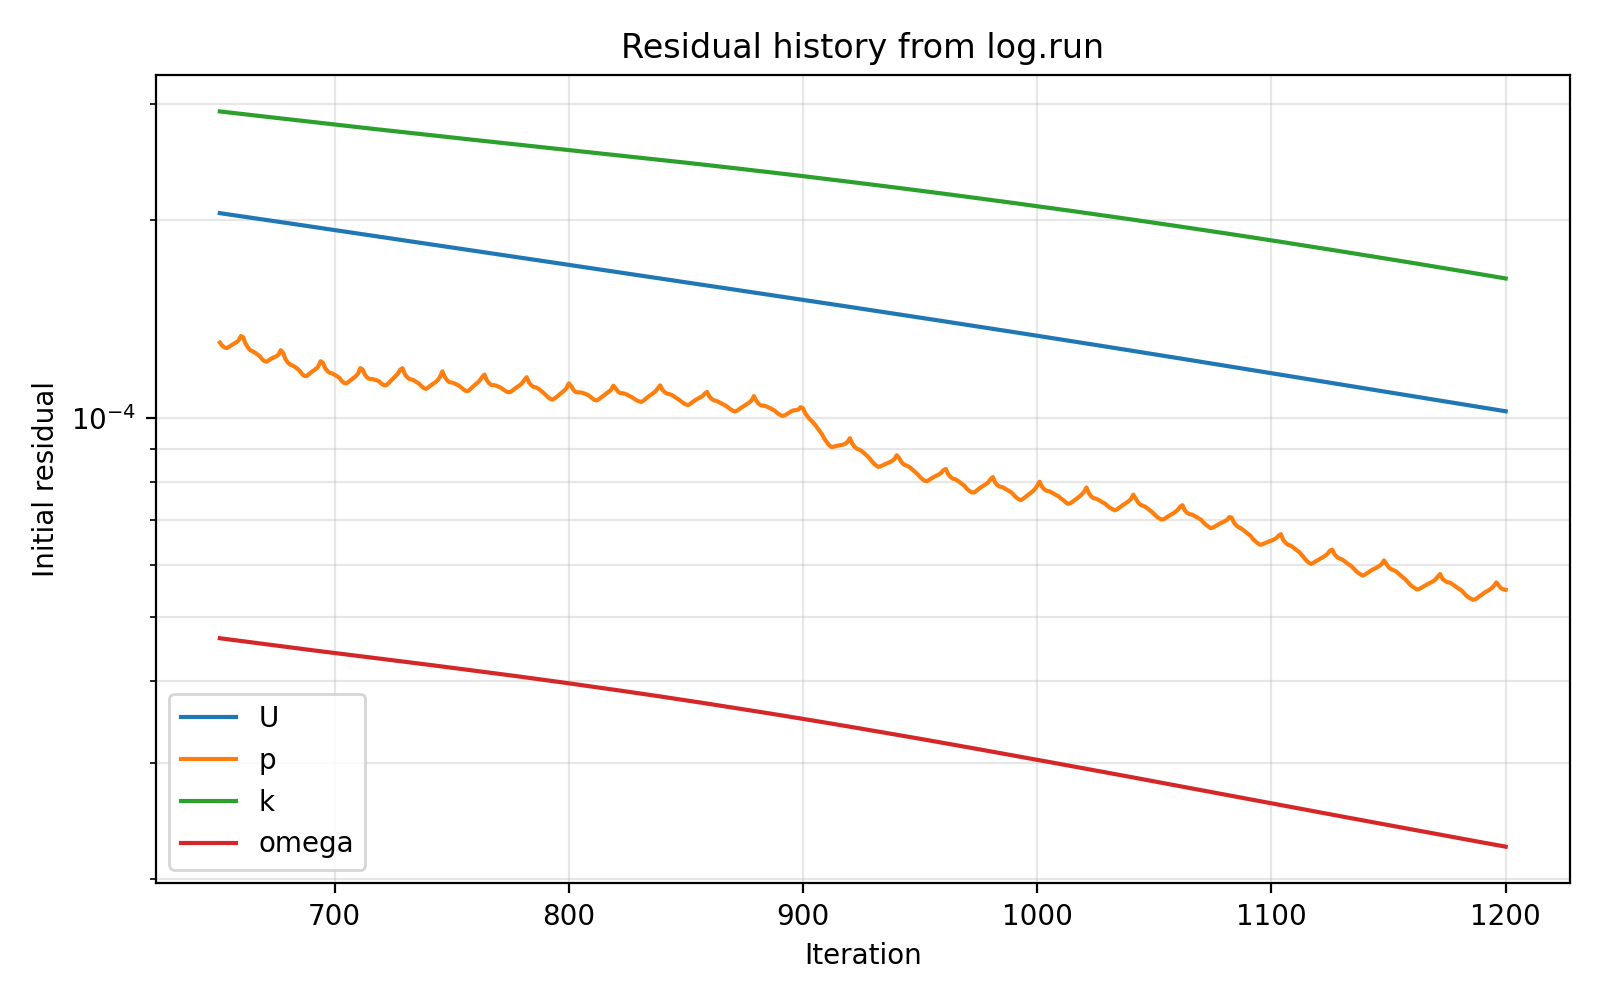
\includegraphics[width=0.95\linewidth]{../docs/figures/residual_history.png}
\caption{Residual history parsed from \texttt{log.run}.}
\end{figure}

\begin{figure}[H]
\centering
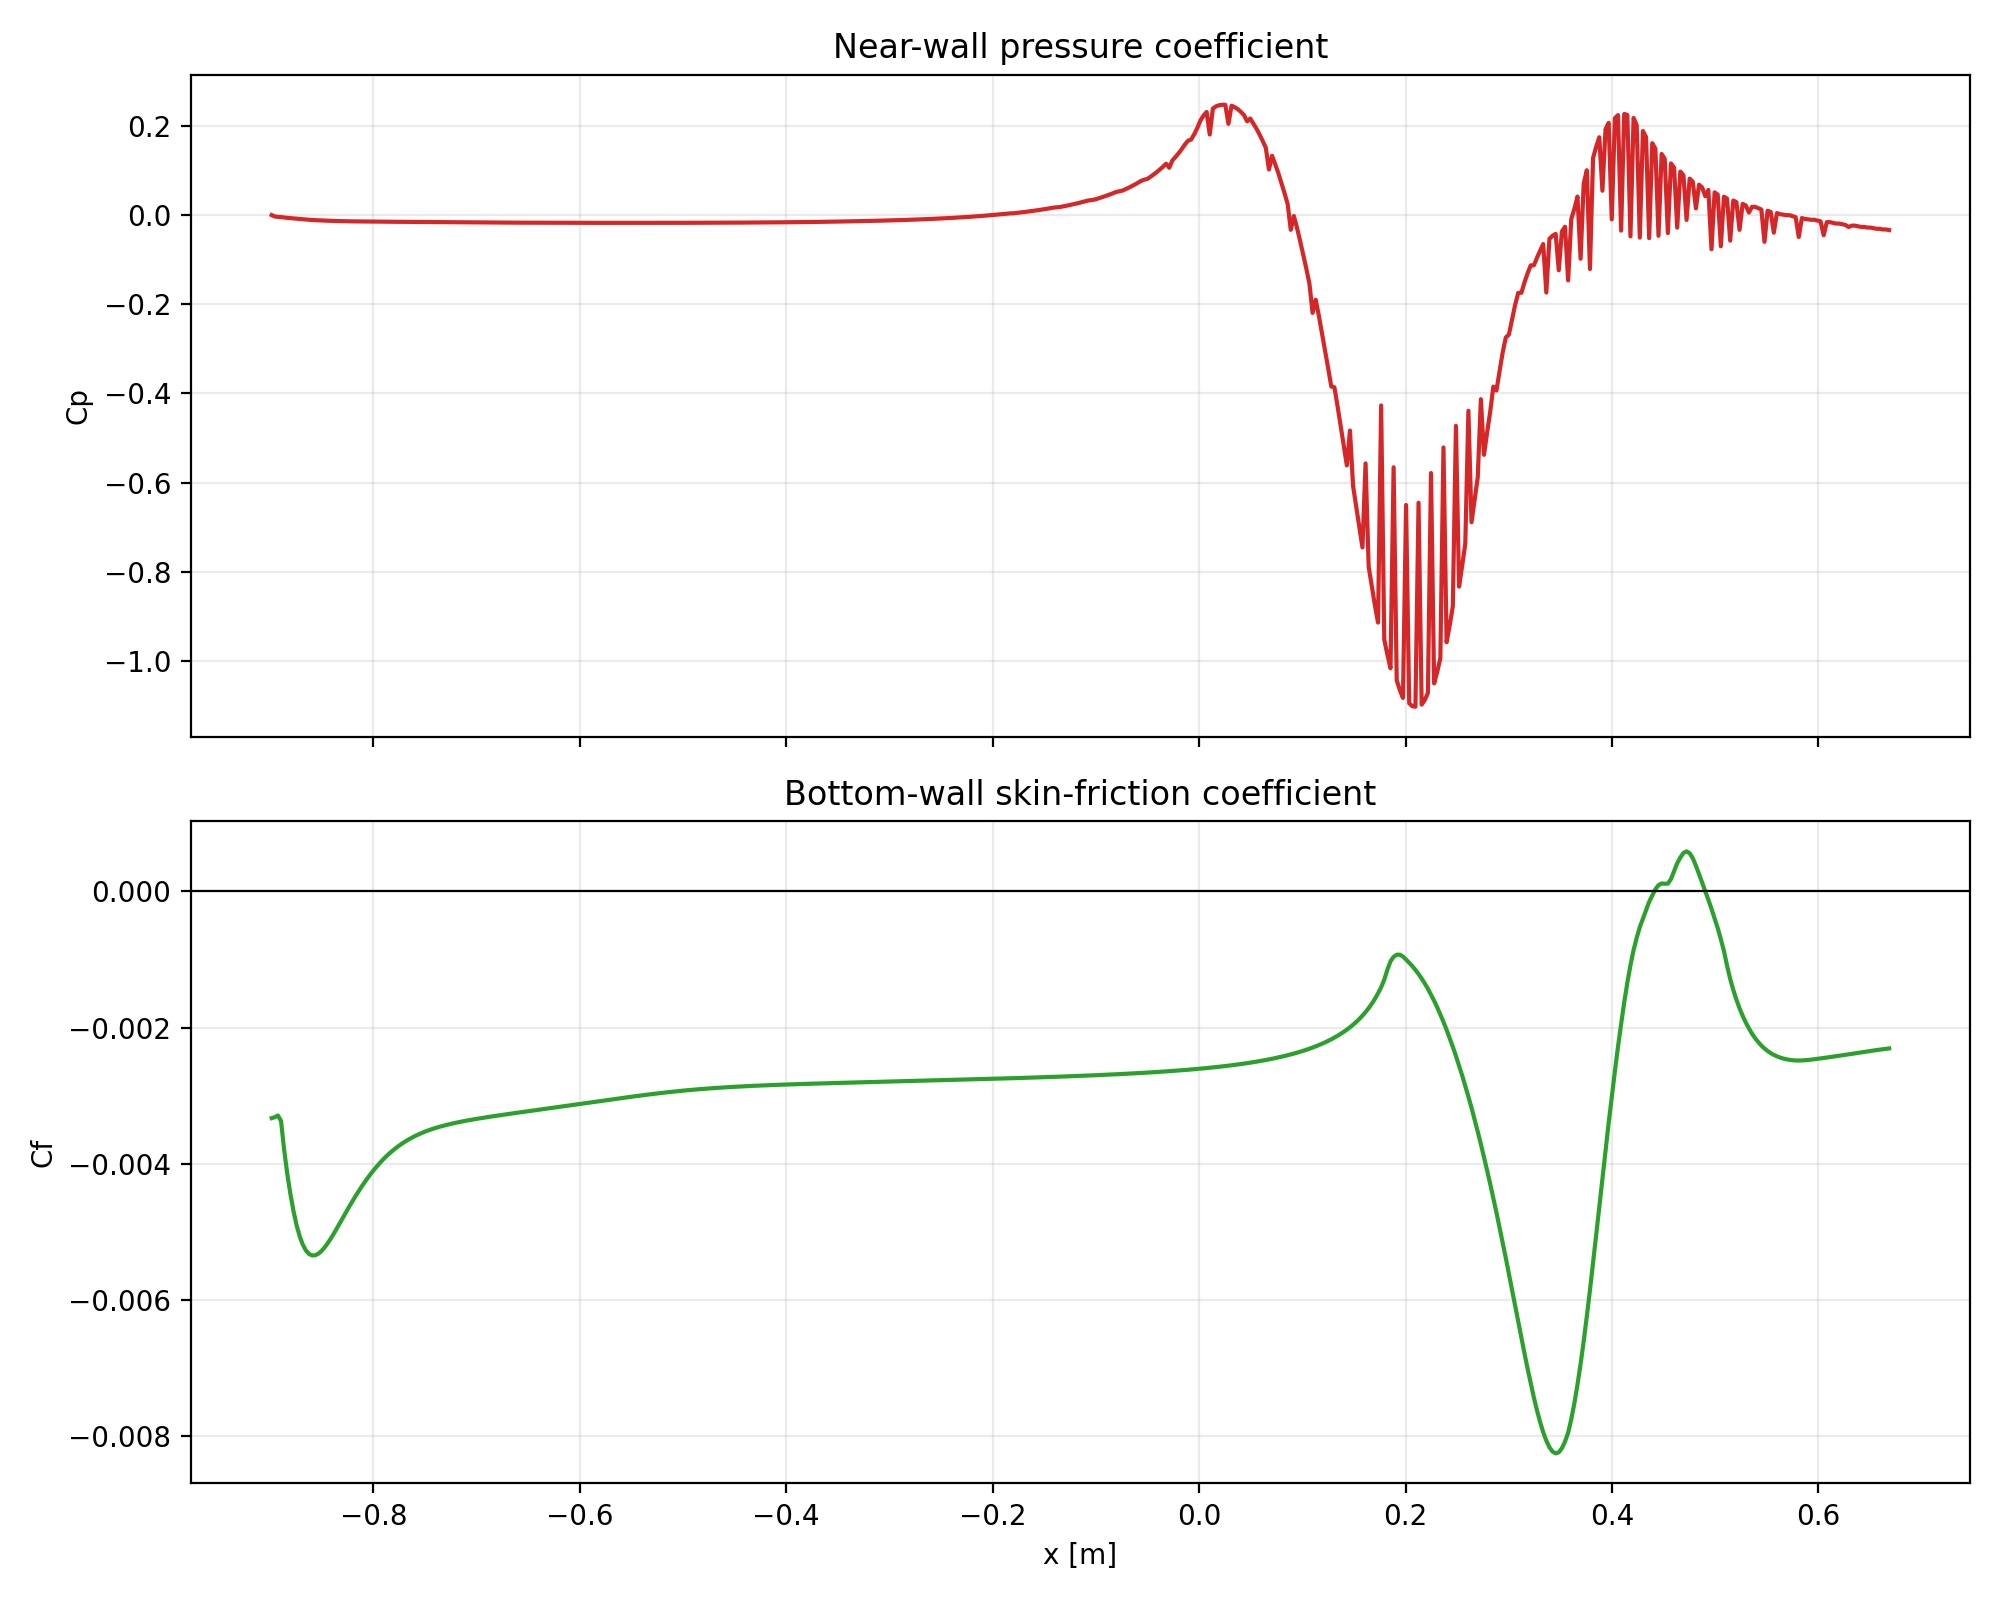
\includegraphics[width=0.95\linewidth]{../docs/figures/wall_coefficients.png}
\caption{Near-wall pressure and skin-friction coefficients derived from the solved field and the wall-shear boundary output.}
\end{figure}

\begin{figure}[H]
\centering
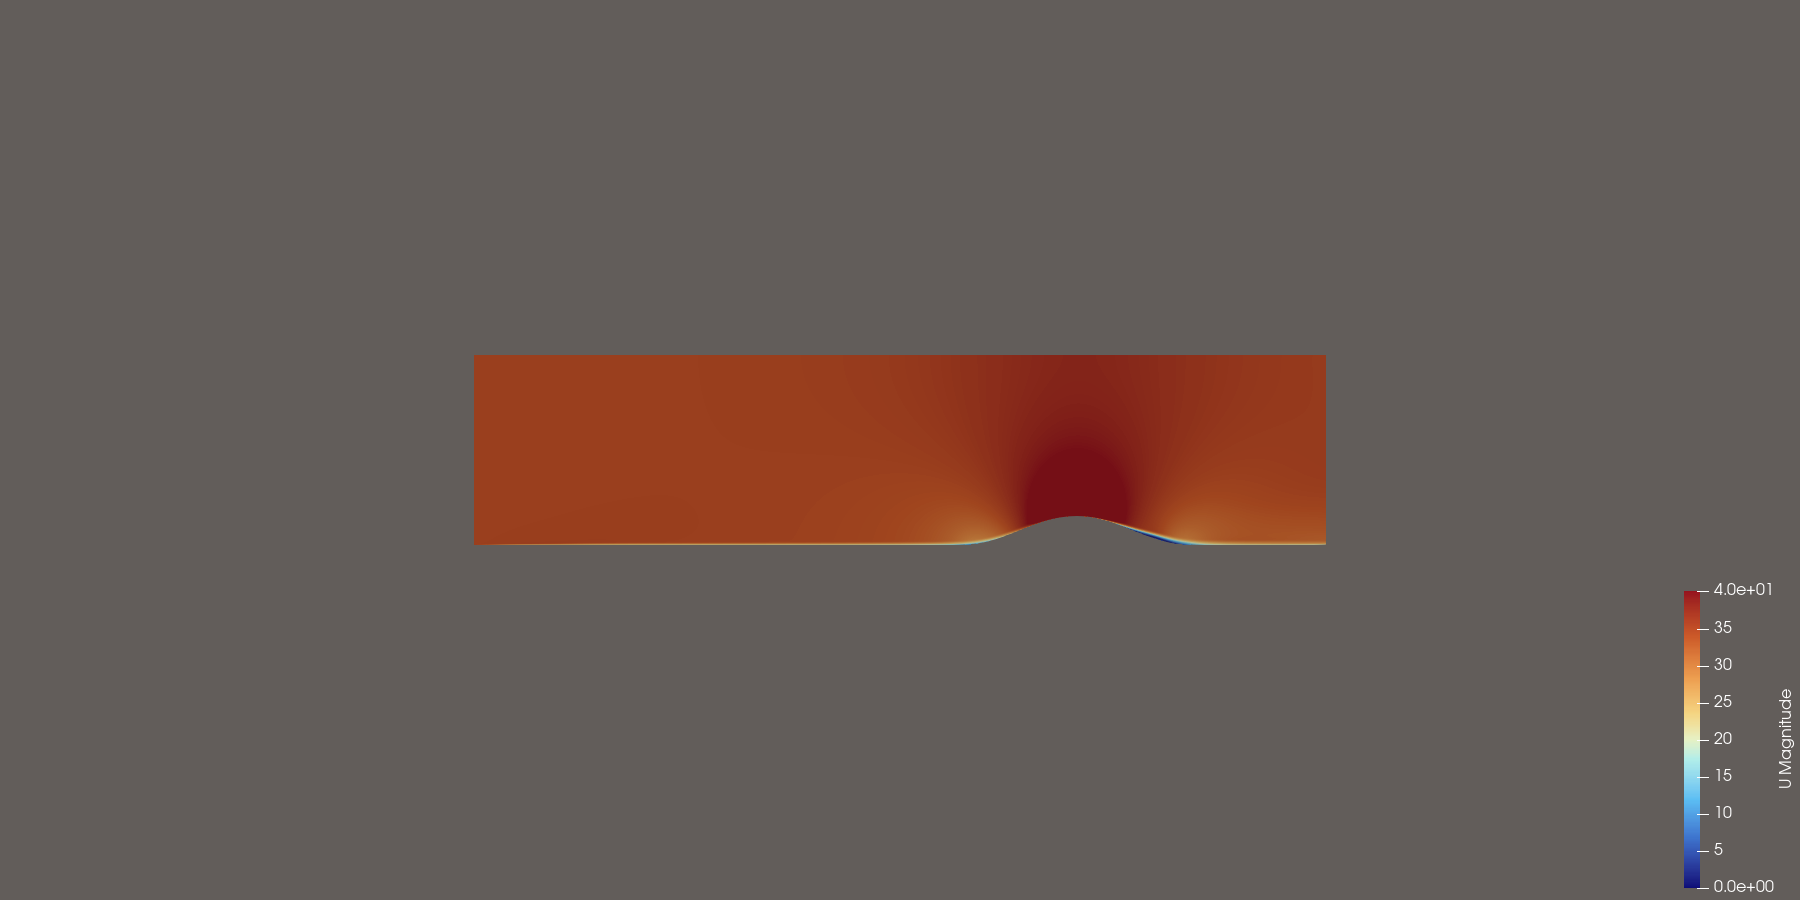
\includegraphics[width=0.95\linewidth]{../docs/figures/paraview_velocity.png}
\caption{ParaView rendering of the internal field colored by velocity magnitude.}
\end{figure}

\begin{figure}[H]
\centering
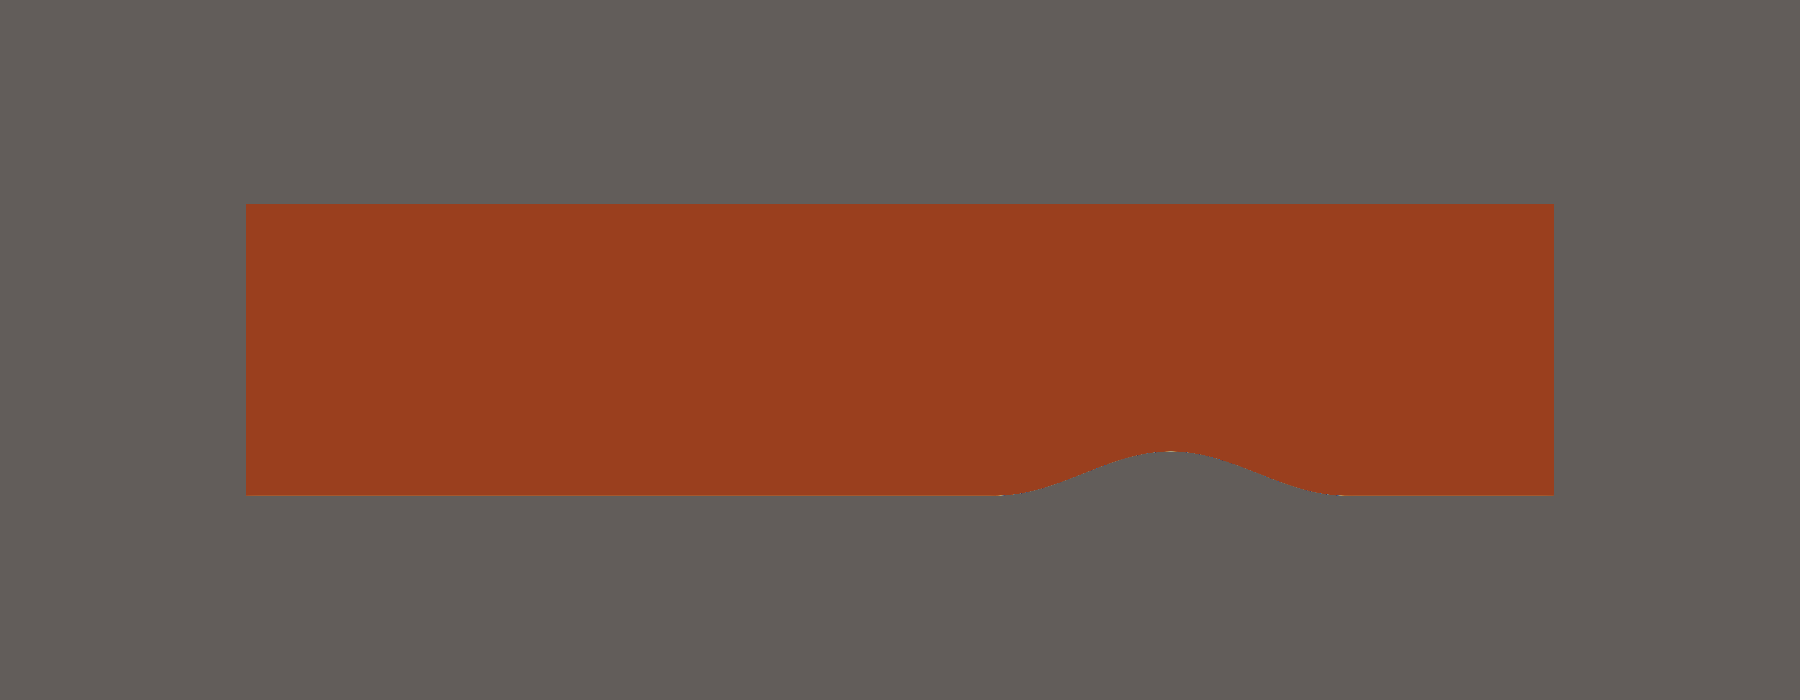
\includegraphics[width=0.95\linewidth]{../docs/figures/paraview_velocity_surface.png}
\caption{ParaView surface-style velocity rendering for a cleaner presentation of the hump-region acceleration pattern.}
\end{figure}

\begin{figure}[H]
\centering
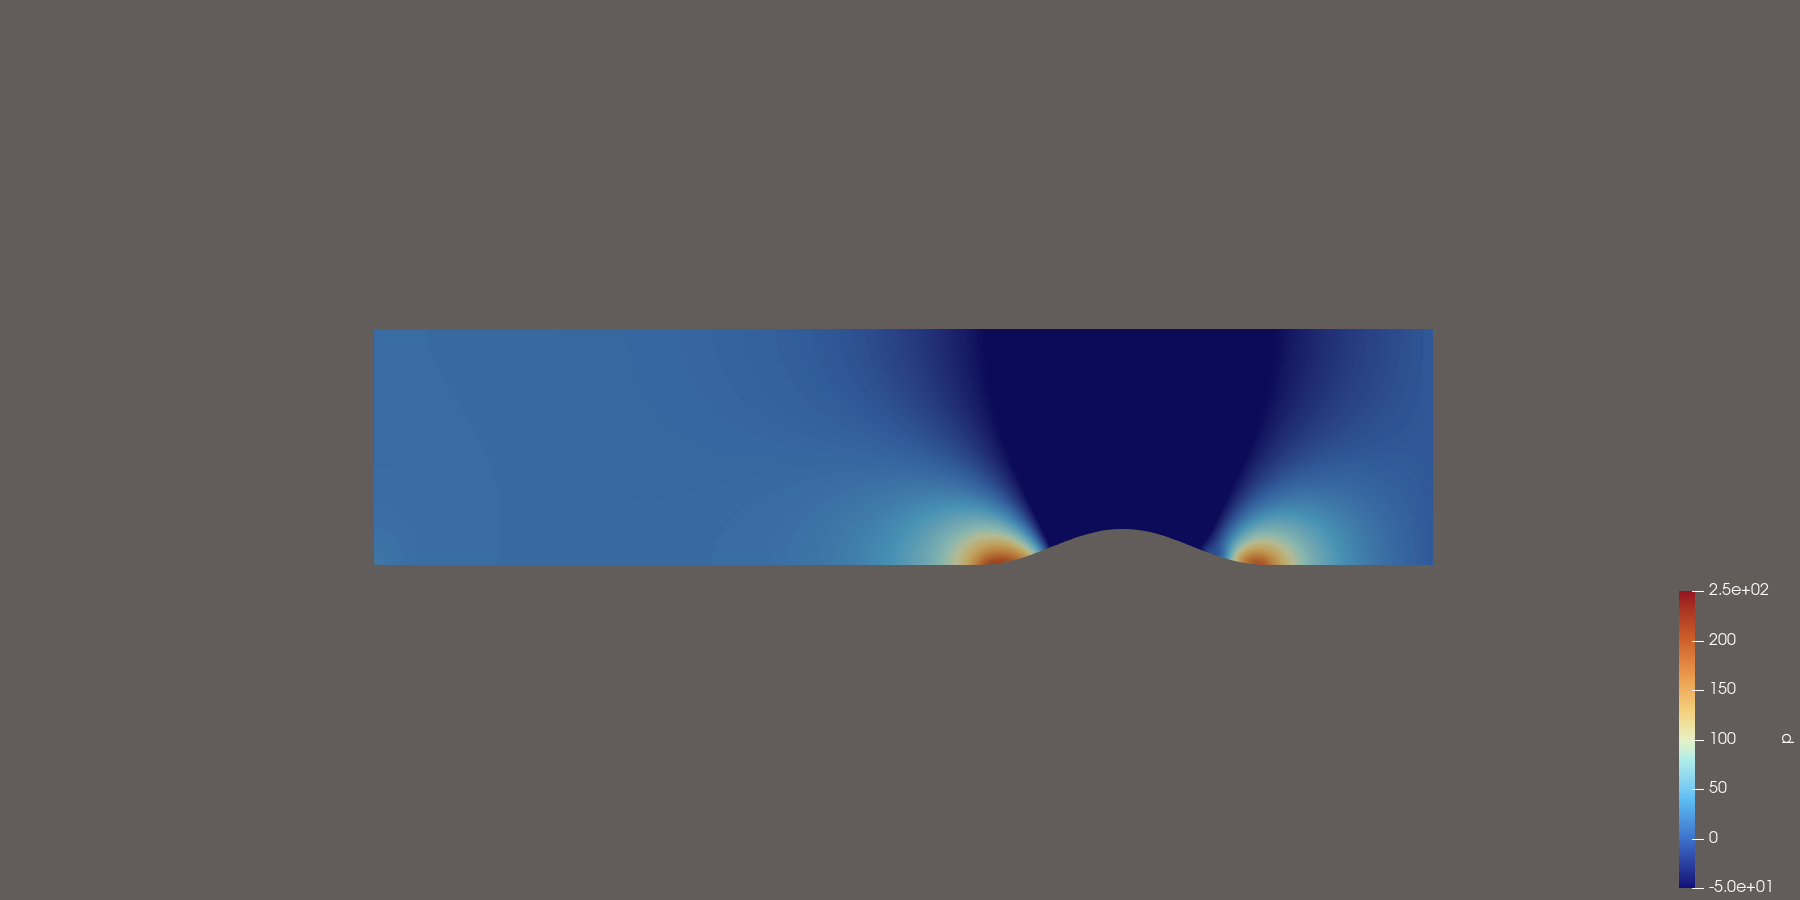
\includegraphics[width=0.95\linewidth]{../docs/figures/paraview_pressure.png}
\caption{ParaView rendering of the internal field colored by pressure.}
\end{figure}

\begin{figure}[H]
\centering

\includegraphics[width=0.95\linewidth]{../docs/figures/paraview_pressure_surface.png}
\caption{ParaView surface-style pressure rendering emphasizing the pressure rise over the hump crest.}
\end{figure}

\begin{figure}[H]
\centering
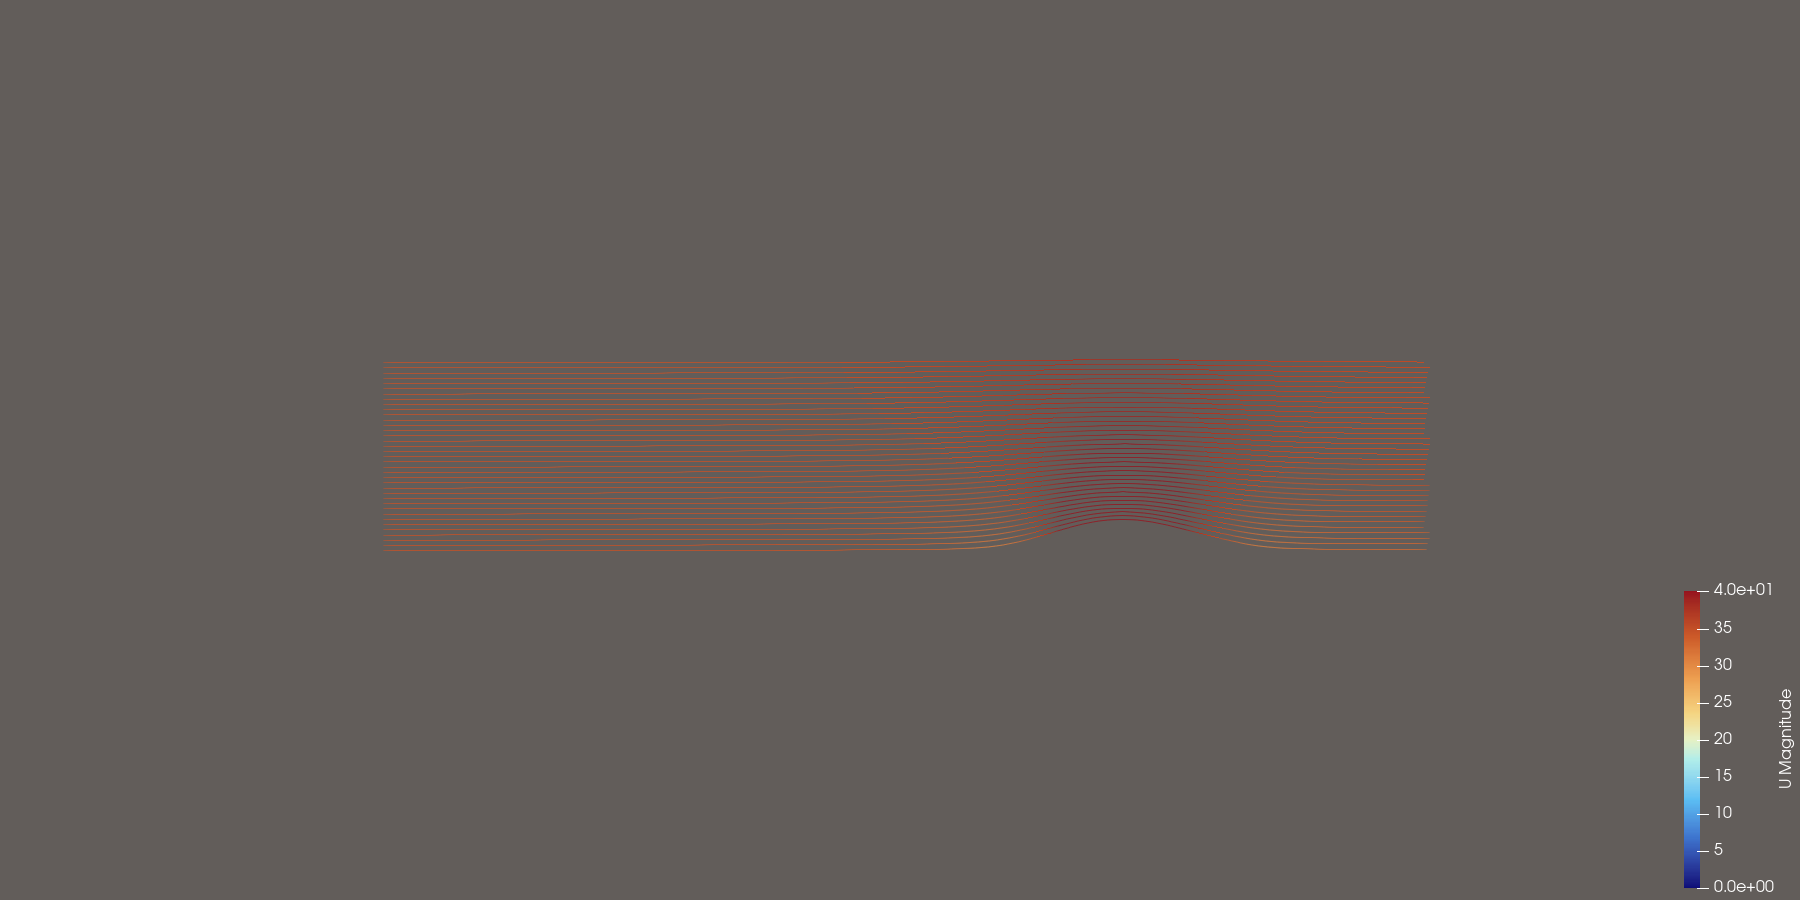
\includegraphics[width=0.95\linewidth]{../docs/figures/paraview_streamlines.png}
\caption{ParaView streamline rendering seeded upstream of the hump.}
\end{figure}

\begin{figure}[H]
\centering
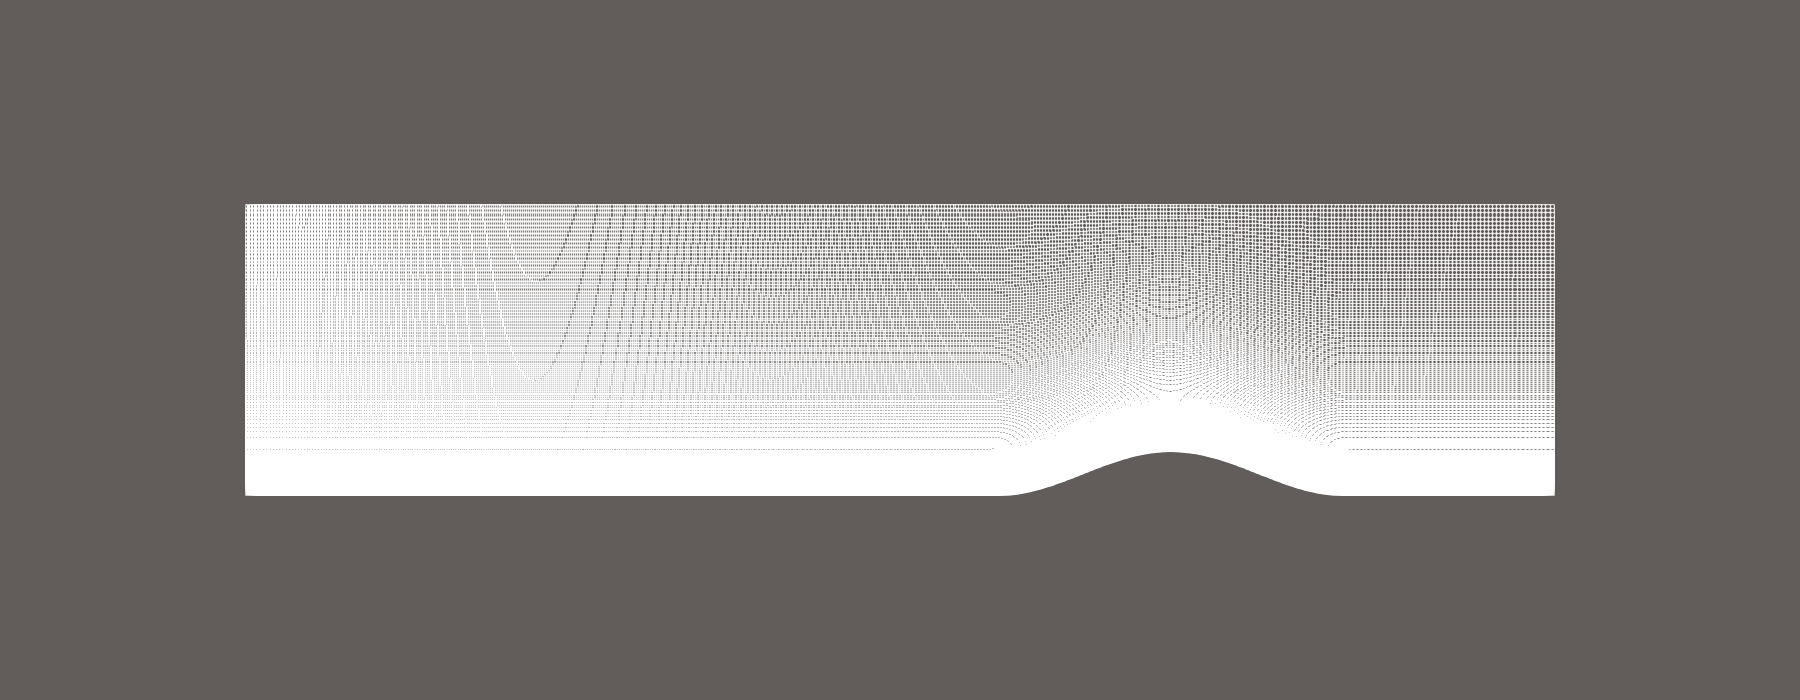
\includegraphics[width=0.95\linewidth]{../docs/figures/paraview_mesh_wireframe.png}
\caption{ParaView wireframe view showing the resolved hump geometry and structured mesh topology.}
\end{figure}

\begin{figure}[H]
\centering
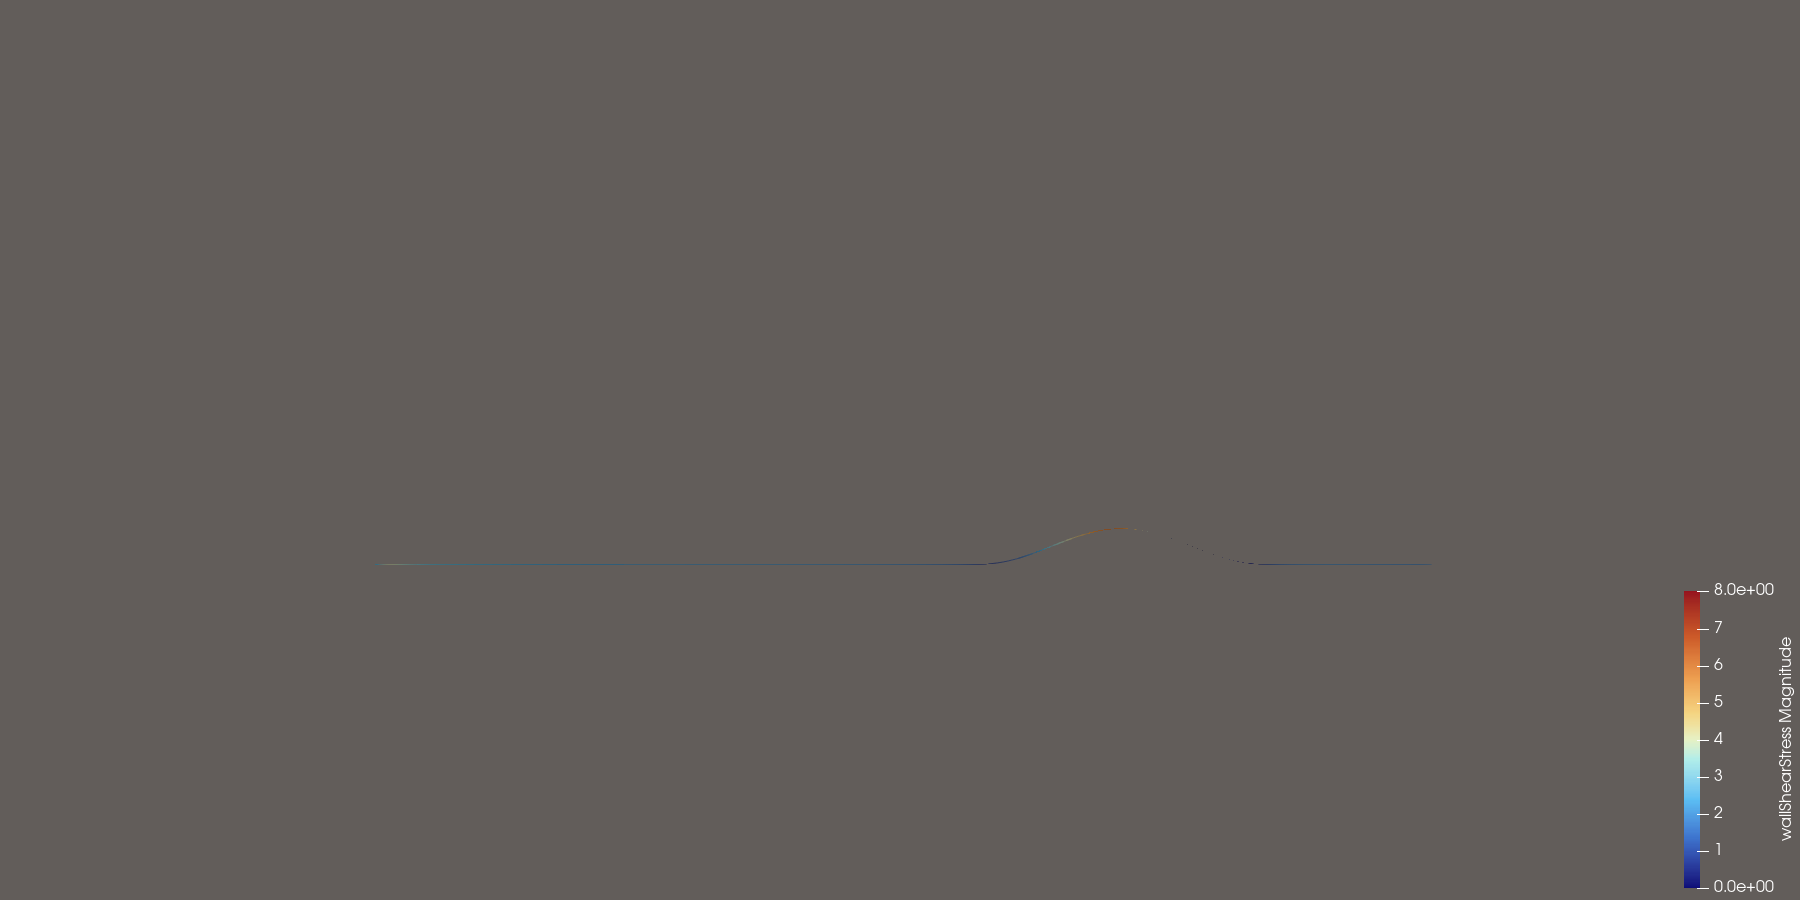
\includegraphics[width=0.95\linewidth]{../docs/figures/paraview_wall_shear.png}
\caption{ParaView rendering of the bottom-wall surface colored by wall-shear magnitude.}
\end{figure}

\section{Results Discussion}
The reconstructed baseline solved stably through 80 SIMPLE iterations and produced coherent velocity and pressure fields plus wall-shear output. The final parsed initial residuals were approximately \(1.79\times 10^{-3}\) for \(U\), \(9.59\times 10^{-3}\) for \(p\), \(2.40\times 10^{-3}\) for \(k\), and \(5.75\times 10^{-4}\) for \(\omega\). This is not a fully converged validation-grade solution, but it is a credible first baseline generated entirely from allowed inputs.

\section{Limitations and Uncertainties}
The main limitations are:
\begin{itemize}
\item the hump geometry is an original smooth reconstruction, not a recovered coordinate set;
\item the top boundary is flat rather than a recovered tunnel contour;
\item the inlet boundary layer is approximated with uniform freestream turbulence quantities;
\item the 80-iteration run is intentionally short, so separation and reattachment indicators remain unresolved in the current baseline;
\item some post-processing uses field-derived approximations rather than the exact original validation pipeline.
\end{itemize}

\section{Reproducibility Instructions}
From the repository root:
\begin{lstlisting}[language=bash]
bash scripts/build_nasa_hump_case.sh
bash scripts/run_nasa_hump_case.sh
bash scripts/postprocess_nasa_hump_case.sh
bash scripts/make_figures.sh
bash scripts/build_report.sh
\end{lstlisting}

The LaTeX source is complete, but this workspace does not currently have \texttt{latexmk} or \texttt{pdflatex}, so \texttt{build\_report.sh} will only succeed after a TeX toolchain is installed.

\section{File-by-File Explanation}
\begin{longtable}{p{0.30\linewidth} p{0.62\linewidth}}
\toprule
File & Role \\
\midrule
\endhead
\texttt{NO\_CHEAT\_PLAN.md} & Compliance guardrails and ordered plan before any edits. \\
\texttt{CASE\_PATTERN\_SUMMARY.md} & Summary of patterns inferred from surviving cases. \\
\texttt{data/NASA\_2DWMH/caseDef} & Central physical parameters used for documentation and consistency. \\
\texttt{data/NASA\_2DWMH/fieldDef} & Shared field groups used by function-object style dictionaries. \\
\texttt{data/NASA\_2DWMH/0/*} & Initial and boundary conditions for \(U\), \(p\), \(k\), \(\omega\), and \(\nu_t\). \\
\texttt{data/NASA\_2DWMH/constant/transportProperties} & Kinematic viscosity chosen from the allowed Reynolds number, chord, and freestream speed. \\
\texttt{data/NASA\_2DWMH/constant/turbulenceProperties} & Baseline SST RANS model selection. \\
\texttt{data/NASA\_2DWMH/system/blockMeshDict} & Generated structured mesh dictionary with spline-defined bottom wall. \\
\texttt{data/NASA\_2DWMH/system/controlDict} & Solver selection, write schedule, and runtime function registration. \\
\texttt{data/NASA\_2DWMH/system/fvSchemes} & Spatial discretization and steady-state declaration. \\
\texttt{data/NASA\_2DWMH/system/fvSolution} & Linear solvers, SIMPLE settings, and relaxation factors. \\
\texttt{data/NASA\_2DWMH/system/singleGraph\_*} & Station definitions corresponding to the chosen \(x/c\) values. \\
\texttt{scripts/generate\_nasa\_hump\_blockmesh.py} & Reproducible authored geometry and mesh generator. \\
\texttt{scripts/build\_nasa\_hump\_case.sh} & Clean rebuild, blockMesh, checkMesh, and cell-center generation through Docker. \\
\texttt{scripts/run\_nasa\_hump\_case.sh} & Dockerized baseline solver execution. \\
\texttt{scripts/postprocess\_nasa\_hump\_case.sh} & Wall-shear and VTK generation through Docker. \\
\texttt{scripts/make\_nasa\_hump\_figures.py} & Direct parsing of fields and logs into CSV data plus plots. \\
\texttt{RECONSTRUCTION\_AUDIT.md} & Final compliance, command, assumption, and output audit. \\
\bottomrule
\end{longtable}

\section{Final Audit Summary}
The final audit is recorded in \texttt{RECONSTRUCTION\_AUDIT.md}. In short, the case was rebuilt from allowed sources only, run through Dockerized OpenFOAM, and documented with explicit assumptions and limitations.

\bibliographystyle{plain}
\bibliography{references}

\end{document}
